\chapter{超伝導}
超伝導の現象論であるGinzburg-Landau理論とBCS理論を扱う. 
\section{超電導の基礎}
\subsection{超電導体の性質}
\begin{itemize}
\item 電気抵抗ゼロ
\item 磁束の侵入を許さない (flux exclusion)
\item 磁束の排除が起こる (flux expulsion)
\end{itemize}
超伝導でない抵抗ゼロの金属ではflux expulsionはない.
\subsection{磁束の量子化}
磁束の量子化は超伝導の巨視波動関数$\psi = \psi_0e^{i\theta}$の一価性の要請から導かれる.
\begin{eqnarray}
  \nonumber  \bm{J}_s &=& \frac{e}{2m}\frac{\hbar}{i}(\psi^*\nabla) - \frac{e^2}{m}|\psi|^2\bm{A}\\
  &=& -\frac{e}{m}|\psi|^2(\hbar\nabla\theta + e\bm{A})
\end{eqnarray}
$\bm{J}_s ~ n_se\bm{v}_s = |\psi|^2e\bm{v}_s$であることに着目すると
\begin{eqnarray}
  \nabla\theta = -\frac{m}{\hbar}\bm{v}_s - \frac{e}{\hbar}\bm{A}
\end{eqnarray}
となる. 波動関数の一価性が保証されるには, 閉曲面$C$に沿って線積分したものが$2\pi$の整数倍でなければならない:
\begin{eqnarray}
  \int_C dl \nabla\theta = \int_C dl \bm{v}_s = 2\pi n
\end{eqnarray}
循環が量子化されている.
\section{超伝導の現象論 : Ginzburg-Landau理論}
超伝導を現象論的にモデル化したGinzburg-Landau理論について. 
\subsection{相転移とOder parameter}
ハミルトニアンが
\begin{eqnarray}
  H = -2\sum_{i,j}J\bm{s}_i\cdot\bm{s}_j
\end{eqnarray}
と書けるようなスピン相互作用を考える. これをハイゼンベルグ模型という. 系の平衡状態はHelmholtz自由エネルギー
\begin{eqnarray}
  F = U -TS
\end{eqnarray}
を最小にするように決まる. 低温($T<\!<U/S$)ならば内部エネルギー$U=\expval{H}$がleadingであり, これを最小化するようにスピンの向きが揃う. これを強磁性体と呼ぶ.  一方で高温ならばエントロピーの項が優勢なのでエントロピーが最大になるようにスピンの向きがバラバラになる. これを常磁性体と呼ぶ.

スピンの向きが揃うときに真空期待値が値を持ち, これを秩序変数と呼ぶ. 秩序変数がゼロでない値に変化するとき, これを相転移と呼ぶ.
\subsection{Ginzburg-Landau方程式}
自由エネルギーを秩序変数$\psi$の冪で展開:
\begin{eqnarray}
  {\cal F}[\psi] = {\cal F}_0 + \alpha|\psi|^2 + \frac{\beta}{2}|\psi|^4
\end{eqnarray}
ここで$\alpha = a(T-T_C)$である. 自由エネルギーの最小を与える$|\psi|$は微分すれば
\begin{eqnarray}
  |\psi| =
  \begin{cases}
    \hspace{1cm}0&(T>T_C)\\
    \\
    \sqrt{\cfrac{a(T_C-T)}{\beta}}&(T<T_C)
  \end{cases}
\end{eqnarray}
と求められる. そもそも$|\psi| = M$(磁化)と考えるのが自然で, なおかつ時間反転対称性を持っているので$M$の奇数次はない. $\alpha<0$のときに$|\psi| = 0$以外の極値を持つようになる. $\alpha(T) = a(T-T_C)$とすれば相転移を記述できる.

$\psi$が空間一様でない, つまり$\psi$が$r$依存性を持つ場合は
\begin{eqnarray}
  {\cal F} &=& {\cal F}_0 + \int d\bm{r} f(\bm{r})\\
  &=& {\cal F}_0 + \int dV\left[\alpha|\psi(\bm{r})|^2 + \frac{\beta}{2}|\psi(\bm{r})|^4\right]  
\end{eqnarray}
と書くことにする. 外部磁場などがある場合, 粒子の運動エネルギ^による補正項を加えなければならない:
\begin{eqnarray}
  \int dV \frac{\hbar^2}{2m}|\nabla\psi(\bm{r})|^2
\end{eqnarray}
自由エネルギーにはゲージ対称性があるので, ゲージ変換に対して不変な形で導入しなければならない:
\begin{eqnarray}
  {\cal F} &=& {\cal F}_0 + \int dV\left[\frac{\hbar^2}{2m}\left|\left(\nabla - \frac{ie}{\hbar}\bm{A}(\bm{r}))\psi(\bm{r}\right)\right|^2 + \alpha|\psi(\bm{r})|^2 + \frac{\beta}{2}|\psi(\bm{r})|^4 + \frac{\mu_0}{2}(\nabla\times\bm{A})^2\right]
\end{eqnarray}
これの変分がゼロになるところを探す:
\begin{eqnarray}
  \nonumber  \delta{\cal F} &=&\int dV\left[-\frac{\hbar^2}{2m}\left(\nabla - \frac{ie}{\hbar}\bm{A}(\bm{r})\right)^2\psi(\bm{r}) + \alpha\psi(\bm{r}) + \beta|\psi(\bm{r})|^2\psi(\bm{r})\right]\delta\psi^*(\bm{r})\\
  &+&\int \left[\frac{\hbar^2}{2m}\left(\nabla - \frac{ie}{\hbar}\bm{A}(\bm{r})\right)\psi(\bm{r})\right]\delta\psi^*(\bm{r})\cdot d\bm{S}
\end{eqnarray}
右辺第一項の被積分関数がゼロになることから
\begin{eqnarray}
  \left[-\frac{\hbar^2}{2m}\left(\nabla - \frac{ie}{\hbar}\bm{A}(\bm{r})\right)^2 + \alpha + \beta|\psi(\bm{r})|^2\right]\psi(\bm{r}) = 0\label{GL}
\end{eqnarray}
を得る. これが秩序変数を記述するGinzburg-Landau(GL)方程式である. ちなみに今回は${\cal F}$について$\psi$の変分を取ったが, $A$についての変分を取るとアンペールの法則が出てくる.
\subsection{ゲージ変換の復習}
\subsubsection{Maxwell方程式}
電磁気学におけるゲージ変換のおはなし. Maxwell方程式
\begin{eqnarray}
  {\rm rot} \bm{E} + \frac{\partial\bm{B}}{\partial t} &=& 0\hspace{2cm}(ファラデーの法則)\\
  {\rm rot} \bm{B} - \varepsilon_0\mu_0\frac{\partial \bm{E}}{\partial t} &=& \mu_0 \bm{i}\hspace{2cm}(アンペールの法則)\\
  {\rm div} \bm{E} &=& \frac{\rho}{\varepsilon_0}\hspace{2cm}(電荷のガウスの法則)\\
  {\rm div} \bm{B} &=& 0\hspace{2cm}(電荷のガウスの法則)
\end{eqnarray}
について. $\bm{B} = {\rm rot}\bm{A}$という仮定をすると${\rm div}\bm{B} = {\rm div\ rot}\bm{A} = 0$という関係が自明に出てくる(ただし, これは$\bm{A}$に特異点がない場合). この仮定をファラデーの法則に代入:
\begin{eqnarray}
  {\rm rot}(\bm{E} + \frac{\partial \bm{A}}{\partial t}) = 0
\end{eqnarray}
もし
\begin{eqnarray}
  \bm{E} + \frac{\partial \bm{A}}{\partial t} = -{\rm grad}\phi \hspace{0.5cm}\Longrightarrow\hspace{0.5cm} \bm{E} = -{\rm grad}\phi - \frac{\partial \bm{A}}{\partial t}
\end{eqnarray}
という仮定をすればファラデーの法則も自明となる. $\phi$と$A$が導入できればMaxwell方程式がとてもカンタンになる. $\phi$と$A$をまとめて電磁ポテンシャルと呼ぶ. 新しい方程式は
\begin{eqnarray}
  \left(\nabla^2 - \varepsilon_0\mu_0\frac{\partial^2}{\partial t^2}\right)\bm{A} - {\rm grad}\left({\rm div}\bm{A} + \varepsilon_0\mu_0\frac{\partial \phi}{\partial t}\right) &=& -\mu_0\bm{i}\label{max1}\\
  \nabla^2\phi + {\rm div}\frac{\partial \bm{A}}{\partial t} &=& -\frac{\rho}{\varepsilon_0}\label{max2}
\end{eqnarray}
となる.ここで
\begin{eqnarray}
  \bm{A}' = \bm{A} + {\rm grad}\chi
\end{eqnarray}
という量を定義しても, 磁束密度$\bm{B}$は変わらない. その代わり電場は変わってしまうので
\begin{eqnarray}
  \phi' = \phi - \frac{\partial \chi}{\partial t}
\end{eqnarray}
を導入すると全て辻褄が合う. この$(\phi, \bm{A})\mapsto(\phi', \bm{A}')$の変換をゲージ変換と呼び, Maxwell方程式はゲージ不変性を持つ.
\subsubsection{ローレンツゲージ}
(\ref{max1})(\ref{max2})には各々$\phi, \bm{A}$が含まれているので計算がめんどくさい. せめて
\begin{eqnarray}
  {\rm div}\bm{A} + \varepsilon_0\mu_0\frac{\partial \phi}{\partial t} = 0\label{max3}
\end{eqnarray}
となってくれれば(\ref{max1})は
\begin{eqnarray}
  \left(\nabla^2 - \varepsilon_0\mu_0\frac{\partial \phi}{\partial t}\right)\bm{A} = -\mu_0\bm{i}\label{max4}
\end{eqnarray}
のように$\bm{A}$だけの式になり, (\ref{max3})を(\ref{max2})に代入すると
\begin{eqnarray}
  \left(\nabla^2 - \varepsilon_0\mu_0\frac{\partial^2}{\partial t^2}\right)\phi &=& -\frac{\rho}{\varepsilon_0}
\end{eqnarray}
という対称性のとてもよい形になる. (\ref{max3})をローレンツ条件という.
\begin{itembox}[c]{ローレンツゲージにおけるMaxwell方程式}
  \begin{eqnarray}
    \nonumber    \left(\nabla^2 - \varepsilon_0\mu_0\frac{\partial \phi}{\partial t}\right)\bm{A} &=& -\mu_0\bm{i}\\
    \nonumber    \left(\nabla^2 - \varepsilon_0\mu_0\frac{\partial^2}{\partial t^2}\right)\phi &=& -\frac{\rho}{\varepsilon_0}
  \end{eqnarray}
  ただし
  \begin{eqnarray}
    \nonumber    {\rm div}\bm{A} + \varepsilon_0\mu_0\frac{\partial \phi}{\partial t} = 0
  \end{eqnarray}
\end{itembox}
\begin{eqnarray}
  (\phi, \bm{A})\mapsto(\phi', \bm{A}') \Longrightarrow
  \begin{cases}
    \bm{A}' = \bm{A} + {\rm grad}\chi\\
    \phi' = \phi - \cfrac{\partial \chi}{\partial t}
  \end{cases}
\end{eqnarray}

がローレンツ条件(\ref{max3})を満たすような$\chi$が存在すれば, この以上の変形が正当化される. ローレンツゲージによるMaaxwell方程式はローレンツ共変である. 
\subsubsection{クーロンゲージ}
ローレンツ条件に対して
\begin{eqnarray}
  {\rm div}\bm{A} = 0
\end{eqnarray}
という条件を課すと, クーロンの法則と等価なポアソン方程式が導かれることからこれをクーロン条件(クーロンゲージ)と呼ぶ.
\begin{itembox}[c]{クーロンゲージにおけるMaxwell方程式}
  \begin{eqnarray}
    \nonumber   && \nabla^2\phi = -\frac{\rho}{\varepsilon_0}\\
    \nonumber    &&\nabla^2\bm{A} -\varepsilon_0\mu_0\frac{\partial^2 \bm{A}}{\partial t^2} - \varepsilon_0\mu_0\frac{\partial}{\partial t}{\rm grad}\phi = \mu_0\bm{i}
  \end{eqnarray}
  ただし
  \begin{eqnarray}
    \nonumber    {\rm div}\bm{A} = 0
  \end{eqnarray}
\end{itembox}
クーロンゲージはローレンツ共変ではなくあまり方程式の対称性は良くないが, 電磁場の量子化などでは便利なので用いられることがある.
\subsection{GLコヒーレンス長と侵入長}
外部磁場がない場合の一次元GL方程式(\ref{GL})を境界条件$\psi(0) = 0$のもとで解く:
\begin{eqnarray}
  \left[-\frac{\hbar^2}{2m}\frac{d^2}{dx^2} + \alpha + \beta|\psi(x)|^2\right]\psi(x) = 0  
\end{eqnarray}
これは$x = 0$の境界には超伝導体はなく, $x > 0$を超電導体で占められているような状況である. コヒーレンス長$/xi$を
\begin{eqnarray}
  \xi^2 = \frac{\hbar^2}{2m|\alpha|}
\end{eqnarray}
と定義する. 超伝導状態では$\alpha < 0$である\footnote{こうしないとGLヘルムホルツエネルギーが$\psi>0$の領域で最小値を持たなくなる.}. 両辺を$\psi_0 = \sqrt{|\alpha|/\beta}$を用いて整理して
\begin{eqnarray}
  -\frac{d^2\psi}{dx^2} - \psi + \psi^3 = 0
\end{eqnarray}
を得る. 左辺に$2\frac{d\psi}{dx}$を掛ける:
\begin{eqnarray}
  2\frac{d\psi}{dx}\left[-\frac{d^2\psi}{dx^2} - \psi + \psi^3\right] = 0
\end{eqnarray}
ここで
\begin{eqnarray}
  \frac{d}{dx}\left(\frac{d\psi}{dx}\right)^2 = 2\frac{d\psi}{dx}\left(\frac{d^2\psi}{dx^2}\right), \hspace{0.5cm}\frac{d\psi^2}{dx} = 2\psi\frac{d\psi}{dx}, \hspace{0.5cm}\frac{d\psi^4}{dx} &=& 4\psi^3\frac{d\psi}{dx}
\end{eqnarray}
を用いて変形する:
\begin{eqnarray}
  \frac{d}{dx}\left[-\xi^2\left(\frac{d\psi}{dx}\right)^2-\psi^2 + \frac{1}{2}\psi^4\right] = 0
\end{eqnarray}
微分がゼロなので微微分関数は定数:
\begin{eqnarray}
  -\xi^2\left(\frac{d\psi}{dx}\right)^2-\psi^2 + \frac{1}{2}\psi^4 = A\ ({\rm const})
\end{eqnarray}
また, 境界条件$d\psi/dx\rightarrow 0, \psi\rightarrow 1\ (x\rightarrow+\infty)$を課すと$A = -\frac{1}{2}$であることがわかる. これにより
\begin{eqnarray}
  \xi^2\left(\frac{d\psi}{dx}\right)^2 = \frac{1}{2}\left(1-\psi^2\right)
\end{eqnarray}
という方程式が得られる.

これは非線形微分方程式だが特解を持っている:
\begin{eqnarray}
  \psi(x) = \tanh(\frac{x}{\sqrt{2\xi}})
\end{eqnarray}
これはソリトン解と呼ばれる. $x = 0$で強制的にゼロにされた$\psi$が$\xi$程度で回復している.また
\begin{eqnarray}
  \xi = \left(\frac{\hbar^2}{2m|\alpha|}\right)^{\frac{1}{2}} = \left(\frac{\hbar^2}{2ma(T-T_C)}\right)^{\frac{1}{2}} = \left(\frac{\hbar^2}{2maT_C}\right)^{\frac{1}{2}}\left(1 - \frac{T}{T_C}\right)^{\frac{1}{2}}
\end{eqnarray}
$T\rightarrow T_C\ (T_C > T)$でコヒーレンス長は発散していく自然な結果が得られる.
\subsection{ソリトンの特徴}
普通の線形波なら波動方程式で記述される異なる波長を持つ波の重ね合わせで記述できる. 異なる波長の波は$v = f\lambda$に従って伝搬速度も異なるので, 波束は次第に崩壊していく(分散が発散していく). しかしソリトンはある非線形微分方程式の定常解なので形を変えずに伝搬していき, 波束も崩壊しない.
\section{超伝導の微視的理論 : Bardeen-Cooper-Schrieffer理論}
\subsection{金属の基本性質}
一辺$L$の箱に閉じ込められた自由電子について考える. 周期境界条件を課すと, 波動関数は平面波で記述できる:
\begin{eqnarray}
  \psi_{\bm{k}}(\bm{r}) = \frac{1}{\sqrt{L^3}}e^{i\bm{k}\cdot\bm{r}}
\end{eqnarray}
エネルギー分散関係は
\begin{eqnarray}
  \varepsilon_{\bm k} = \frac{\hbar^2k^2}{2m}
\end{eqnarray}
である. ここで波数は
\begin{eqnarray}
  k_i = n_i\left(\frac{2\pi}{L}\right)\hspace{0.5cm}(i= x, y, z)
\end{eqnarray}
で与えられる. 3次元$k$空間の単位体積$(2\pi/L)^3$あたりに1つ(スピン自由度を考えると2つ)の状態が入れる. 下の準位から埋めていくと, 状態が埋まった空間は球になる. これをフェルミ球と呼び, その境界をフェルミ面と呼ぶ. フェルミ面の半径を$k_F$とすると
\begin{eqnarray}
  N = 2\left(\frac{L}{2\pi}\right)^3\times\frac{4}{3}\pi k_F^3
\end{eqnarray}
である. 電子密度を$n = N/L^3$とすると
\begin{eqnarray}
  k_F = (3\pi n)^{\frac{1}{3}}
\end{eqnarray}
となる. エネルギー$\varepsilon$の状態を電子が占める確率はFermi-Dirac分布関数
\begin{eqnarray}
  f(\varepsilon) = \frac{1}{\exp[(\varepsilon- \varepsilon_F)/k_BT]+1}
\end{eqnarray}
で与えられる.
\subsection{電子-格子間相互作用}
電子と金属イオンの間の相互作用は電子がイオン構造を歪めるという描像で理解される\footnote{金属イオン中に電子があると電子と金属イオンが引力相互作用で近づき合い, 金属イオンの配列が微妙に歪むことになる. この電子が金属中を移動すると, 金属イオンの配列の歪みも一緒に伝搬していくように見える. これが格子振動であり, これを量子化するとフォノンになる. さて, この場合は電子の運動エネルギーが格子振動に一部持って行かれることになり, これが電気抵抗の由来になる. しかし, この電子の近くに別の電子がある場合は, 格子振動により正電荷密度が大きくなっているところからさらに引力相互作用を受けて加速することができる. つまり, ある電子が創りだした格子振動エネルギーを別の電子が受け取る, というメカニズムである. もちろんこれば古典的な描像であり, 全ての格子振動エネルギーが別の電子に引き継がれることは一見なさそうだが, 格子振動を量子化したフォノンであればdescreteなエネルギーのやりとりしかできないことになるので, 電子がフォノンのやりとりをすることでエネルギーの散逸を防ぐ枠組みを正当化することができそうである. このフォノンのやり取りをする電子の組をCooper-pairという. }. つまり, 電子がフォノンを放出して異なる波数を持つモードへ遷移する, という描像である. フォノンを介した2電子間相互作用とは, 波数$k_1, k_2$の電子が$k_1 - q, k_2 + q$となる過程である.

\begin{figure}[htbp]
  \begin{minipage}{0.5\hsize}
    \centering
    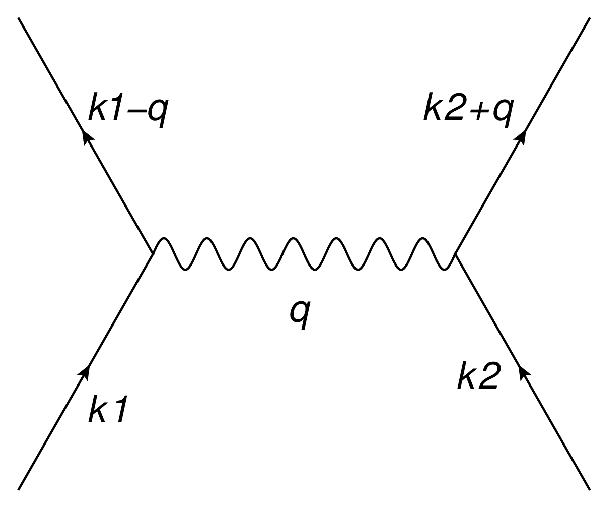
\includegraphics[width = 5.5cm]{./EPS/newdiagram1.eps}
    \figcaption{$\bm{k}_1$がフォノン$\bm{q}$を放出する過程}
    \label{diagram1}
  \end{minipage}
  \begin{minipage}{0.5\hsize}
    \centering
    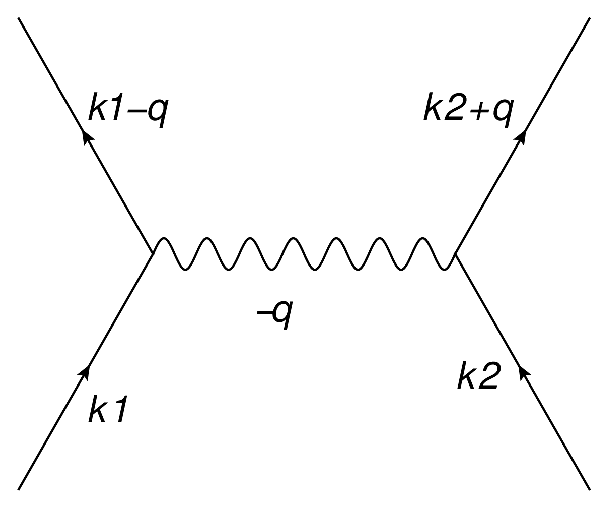
\includegraphics[width = 5.5cm]{./EPS/newdiagram2.eps}
    \figcaption{$\bm{k}_1$がフォノン$\bm{-q}$を吸収する過程}
    \label{diagram2}
  \end{minipage}
\end{figure}
フォノンを介した相互作用ハミルトニアンを$H'$とすると, エネルギーの2次摂動は
\begin{itemize}
\item 同じ電子がフォノンを放出して吸収した場合は自己エネルギー
\item 異なる電子同士がフォノンのやりとりをした場合は相互作用
\end{itemize}
を表すことになる. さて, 上の2種類の過程を考慮すると相互作用項の期待値は
\begin{eqnarray}
  U_2 &=& \sum_m\frac{\bra{f}H'\ket{m}\bra{m}H'\ket{i}}{E_i-E_m}\\
  E_i &=& \varepsilon_{\bm{k}_1} +\varepsilon_{\bm{k}_2}\\
  E_m &=&
  \begin{cases}
    \varepsilon_{\bm{k}_1 - \bm{q}} +\varepsilon_{\bm{k}_2} + \hbar\omega_{\bm{q}}\\
    \varepsilon_{\bm{k}_1} +\varepsilon_{\bm{k}_2 + \bm{q}} + \hbar\omega_{\bm{q}}
  \end{cases}
\end{eqnarray}
より
\begin{eqnarray}
  U_2 &=& \frac{|V_{\bm q}|^2}{\varepsilon_{\bm{k}_1 - \bm{q}} +\varepsilon_{\bm{k}_1} + \hbar\omega_{\bm{q}}} + \frac{|V_{\bm q}|^2}{\varepsilon_{\bm{k}_2} +\varepsilon_{\bm{k}_2 + \bm{q}} + \hbar\omega_{\bm{q}}}\\
  &=& \frac{2|V_{\bm q}|\hbar\omega_{\bm q}}{(\varepsilon_{\bm{k}_1 - \bm{q}} +\varepsilon_{\bm{k}_1})^2-(\hbar\omega_{\bm q})^2}
\end{eqnarray}
となる. ここではエネルギー保存則を用いた. $|\varepsilon_{\bm k} - \varepsilon_{\bm k-q}| <\!< \hbar\omega_{\bm q}$であれば電子間相互作用は引力となる. つまり, フェルミ面上の電子間にはフォノンを介した引力相互作用が働く可能性がある.
\subsection{Cooper問題}
次に問題になるのが, 「フェルミ面直上にある2つの電子間相互作用を考えるとき, この電子対が束縛状態を作るか」ということ. 言い換えると, 「いかに弱くても引力相互作用があれば電子対の束縛状態が実現するかどうか」. 着目する2電子の波動関数を
\begin{eqnarray}
  \Psi(\bm{r}_1, \sigma_1, \bm{r}_2, \sigma_2) = \psi(\bm{r}_1, \bm{r}_2)\chi(\sigma_1, \sigma_2)
\end{eqnarray}
とする. $\psi$が満たすのはScr\"odinger方程式
\begin{eqnarray}
  &&\bqty{-\frac{\hbar^2}{2m}\pqty{\nabla^2_1 + \nabla^2_2} + V(\bm{r}_1, \bm{r}_2)}\psi(\bm{r}_1, \bm{r}_2) = E\psi(\bm{r}_1, \bm{r}_2)\\
  &&\chi(\sigma_1, \sigma_2) = \frac{1}{\sqrt{2}}\pqty{\ket{\uparrow}\ket{\downarrow} - \ket{\downarrow}\ket{\uparrow}}
\end{eqnarray}
重心・相対座標$\bm{R} = \pqty{\bm{r}+\bm{r}}/2,\ \bm{r} = \bm{r}_1 - \bm{r}_2$を用いて
\begin{eqnarray}
  \psi(\bm{r}_1,\bm{r}_2) = \varphi(\bm{r})e^{i\bm{KR}}
\end{eqnarray}

